\documentclass[11pt]{article}
\usepackage{icmlko}
\begin{document}

\title{짝이 없으면 아무것도 못 잰다 --- 이백 편 동안 넷째 자리로 적어 온 수의 첫째 자리를 재다}
\author{월드모델 실험실}
\date{노트 352 · 2026년 8월 1일}
\maketitle

\begin{abstract}
노트 351이 시장팝업 서랍을 비우고 ``다음은 라벨''이라고 적었다. 라벨을
쟀다 --- \texttt{label\_trust} 등급으로 유보를 갈랐더니 \emph{좋은} 등급
(B+C, 82행)이 $\rho=+0.2147$ 로 전체(+0.2880)보다 \textbf{낮았다.}
미리 적은 예측(``B+C가 0.05 이상 높으면 라벨이 병목'')이 반대 방향으로
깨졌다. 퍼짐을 맞춰도, 장소로 갈라도, 무리 안/사이로 분해해도 설명이
안 됐다. 그래서 마지막으로 남은 것을 쟀다 --- \textbf{그 $\rho$ 자체가
얼마나 단단한가.} 유보 행을 재표집한 95\% 구간은 시장팝업
$[0.085,\,0.468]$ · 아이돌 $[0.052,\,0.817]$ · 팝업(\emph{대표 수치})
$[0.257,\,0.660]$ 이다. 도메인 마흔다섯 쌍 중 \textbf{서른일곱 쌍은 순서를
못 가린다.} 판도 수준으로 재면 $0.4953\,[0.4623,\,0.5252]$ 로 SD 0.0161
이다 --- 그런데 \textbf{짝 뽑기 SD 는 0.0031, 다섯 배 작다.} 지난
스물두 편이 +0.003 짜리 걸음을 잴 수 있었던 것은 전부 짝 덕이었다.
시장팝업이 ``자꾸 진다''는 것도 아직 증명된 적이 없다 --- 그 구간은
도서 · 펀딩 · 웹툰과 겹친다.
\end{abstract}

\section{라벨을 쟀다 --- 그리고 반대로 깨졌다}

시장팝업 유보 104행의 \texttt{label\_trust} 등급은 B 41 · C 41 · E 16 ·
D 4 · A 2 다. E 는 ``예상치 재활용 · 추산 표현''이다. 미리 적었다:
\emph{B+C 의 $\rho$ 가 전체보다 0.05 이상 높으면 라벨 잡음이 병목이다.}

\begin{center}
\begin{tabular}{lrrr}
\hline
부분집합 & $n$ & $\rho$ & 같은 크기 무작위 \\
\hline
전체        & 104 & $+0.2880$ & --- \\
B+C         &  82 & $+0.2147$ & $+0.2846$ (SD 0.052) \\
C+D+E       &  61 & $+0.1945$ & $+0.2915$ (SD 0.081) \\
D+E 만      &  20 & $+0.3920$ & $+0.2820$ (SD 0.206) \\
\hline
\end{tabular}
\end{center}

\textbf{깨끗한 라벨이 더 못 맞힌다.} 미리 적어 둔 대로 같은 크기 무작위
부분집합과 견줬기 때문에 ``표본이 작아서''는 아니다. 이어서 셋을 더
지웠다 --- ① 퍼짐: 등급과 라벨은 무관하고(크루스칼 $p=0.32$) $y$ 의
SD 를 맞춘 무작위와 견줘도 B+C 는 여전히 아래다($p=0.848$). ② 장소:
백화점 $+0.2089$ · 몰 $+0.0712$ · 노면 $+0.2473$ --- 셋 다 제 크기의
무작위보다 낮고 서로 안 갈린다. ③ 무리 사이/안: 무리 안에서 다시 순위를
매겨도 $\rho$ 가 안 죽는다(업종 기준 전체 $+0.2986$ → 무리 안
$+0.2693$). 사이가 아니라 안에서 나오는 신호다.

\textbf{남은 설명은 하나뿐이었다.} 이름 붙인 부분집합이 하나같이 제
영분포의 아래쪽 1 SD 근처에 앉는다면, 갈랐기 때문이 아니라 $\rho$ 자체가
몇 행에 얹혀 있어서다. 그래서 갈래를 바꿔 \emph{$\rho$ 의 굳기}를 쟀다.

\section{넷째 자리로 적어 온 것들}

\begin{center}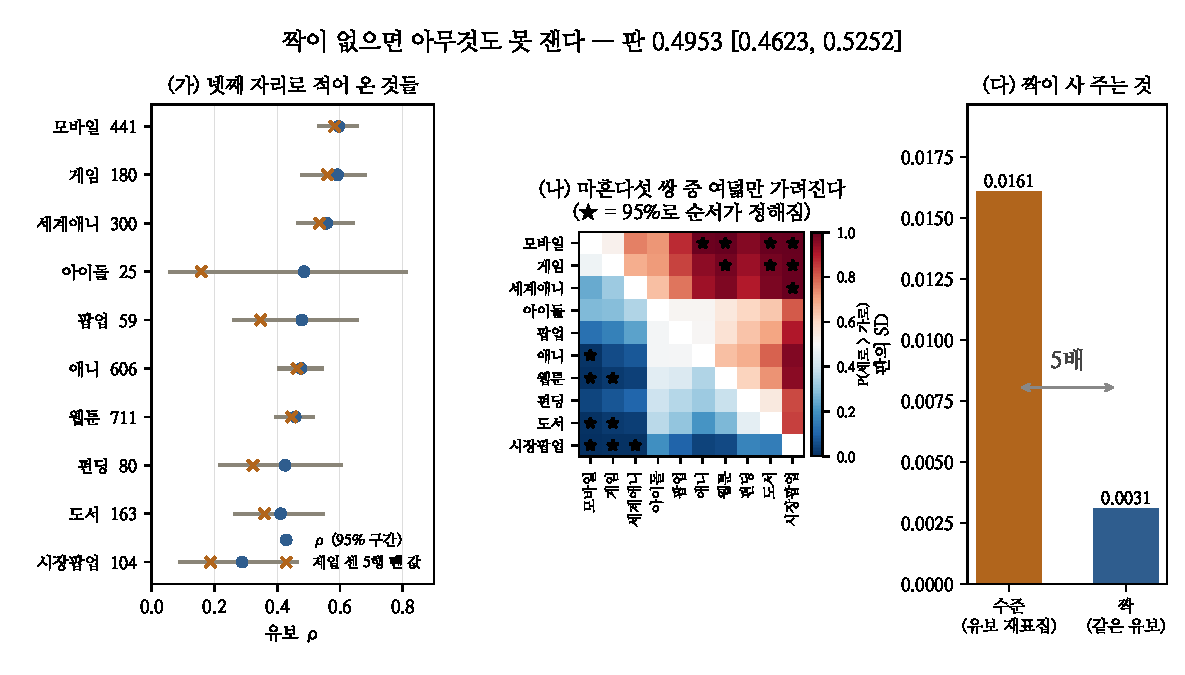
\includegraphics[width=\linewidth]{figs/paired.pdf}\end{center}

유보 행만 재표집한 95\% 구간이다(예측은 고정, 모형은 다시 안 맞춘다).

\begin{center}
\begin{tabular}{lrrrr}
\hline
도메인 & 유보 & $\rho$ & 95\% 구간 & 센 5행 뺀 값 \\
\hline
웹툰     & 711 & $+0.4574$ & $[+0.393,\,+0.520]$ & $+0.4462$ \\
애니     & 606 & $+0.4760$ & $[+0.402,\,+0.549]$ & $+0.4631$ \\
모바일   & 441 & $+0.5962$ & $[+0.530,\,+0.658]$ & $+0.5831$ \\
세계애니 & 300 & $+0.5579$ & $[+0.462,\,+0.646]$ & $+0.5352$ \\
게임     & 180 & $+0.5923$ & $[+0.475,\,+0.685]$ & $+0.5605$ \\
도서     & 163 & $+0.4110$ & $[+0.261,\,+0.551]$ & $+0.3596$ \\
시장팝업 & 104 & $+0.2880$ & $[+0.085,\,+0.468]$ & $+0.1875$ \\
펀딩     &  80 & $+0.4252$ & $[+0.212,\,+0.610]$ & $+0.3229$ \\
\textbf{팝업} &  59 & $+0.4788$ & $[+0.257,\,+0.660]$ & $+0.3477$ \\
아이돌   &  25 & $+0.4860$ & $[+0.052,\,+0.817]$ & $+0.1580$ \\
\hline
\end{tabular}
\end{center}

셋을 읽는다.

\textbf{하나 --- 순위가 거의 안 정해진다.} 마흔다섯 쌍 중 95\%로 순서가
가려지는 것은 \textbf{여덟 쌍}뿐이다(그림 (나)). 큰 셋(모바일 · 게임 ·
세계애니)이 작은 셋(도서 · 시장팝업 · 웹툰 일부)보다 위라는 것 말고는
아무것도 못 말한다. 아이돌 · 팝업 · 펀딩은 \emph{누구와도} 안 갈린다.

\textbf{둘 --- 시장팝업이 진다는 말은 증명된 적이 없다.} 구간
$[0.085,\,0.468]$ 은 도서(0.411) · 펀딩(0.425) · 웹툰(0.457)을 다 덮는다.
노트 351과 그 앞의 몇 편이 ``시장팝업이 왜 자꾸 지나''를 물었는데,
\textbf{그 전제부터 아직 안 재진 것이었다.}

\textbf{셋 --- 대표 수치가 제일 얇은 축에 속한다.} 팝업은 유보 59행이고
구간 폭이 0.40이다. 노트 351이 채택한 걸음은 팝업 $+0.0168$ 이었다 ---
구간 폭의 24분의 1이다. 그 걸음은 \emph{짝}으로 쟀으니 유효하지만,
0.4788 이라는 \emph{수준}을 밖에 내보낼 때는 소수 넷째 자리가 아니라
``0.3\textasciitilde0.7'' 이라고 적어야 맞다.

\section{그런데 루프는 왜 굴러갔나 --- 짝}

판을 수준으로 재면 $0.4953$, 95\% $[0.4623,\,0.5252]$, SD $0.0161$ 이다.
같은 판을 \emph{짝 학습 뽑기}로 재면 SD $0.0031$ --- \textbf{다섯 배
작다}(그림 (다)). 유보를 고정하고 학습만 흔들면 유보 표집 오차가 두 팔에
똑같이 실려 차에서 상쇄되기 때문이다.

이것이 지난 스물두 편의 실제 근거였다. 노트 348의 $+0.0068$, 노트 349의
$+0.0044$, 노트 350의 $+0.0033$, 노트 351의 $+0.0002$ --- 전부 판 수준
SD(0.0161)의 5분의 1 이하다. \textbf{짝을 안 지었으면 넷 다 잡음에
묻혔다.} 규약이 처음부터 짝이었던 것은 운이 좋았다.

\textbf{따라서 규약에 못을 박는다.}
\begin{itemize}
\item \textbf{짝으로 잰 차만 보고한다.} 판이든 도메인이든 수준은
비교에 안 쓴다.
\item \textbf{수준을 적을 때는 구간을 같이 적는다.} 팝업 $0.479$ 가
아니라 $0.479\,[0.26,\,0.66]$ 이다.
\item \textbf{``어느 도메인이 제일 낮은가''는 물으면 안 되는 질문이다}
--- 마흔다섯 쌍 중 서른일곱이 안 갈린다. 낮아 보이는 도메인을 쫓는 대신
\emph{짝으로 오르는 처치}를 쫓는다.
\end{itemize}

\section{그래서 무엇을 해야 하나}

구간을 좁히는 길은 유보를 늘리는 것뿐이고, 폭은 $1/\sqrt{n}$ 로 준다.

\begin{center}
\begin{tabular}{lrrrr}
\hline
도메인 & 지금 $n$ & 폭 & $n\times2$ & $n\times4$ \\
\hline
아이돌   &  25 & 0.756 & 0.535 & 0.378 \\
팝업     &  59 & 0.406 & 0.287 & 0.203 \\
펀딩     &  80 & 0.397 & 0.281 & 0.198 \\
시장팝업 & 104 & 0.400 & 0.283 & 0.200 \\
\hline
\end{tabular}
\end{center}

\textbf{아이돌 26행이 서랍에 있다}(노트 326에서 넓히며 유보에는 안 넣은
것). 유보 $25\to51$ 이면 폭 $0.756\to0.535$ 다. 지금까지 이 갈래를
``과제가 바뀌므로 미룬다''로 미뤄 왔는데, 과제가 바뀌는 대가로 사는 것이
구간 폭 0.22 라면 사는 쪽이 맞다. \textbf{다음에 이것을 한다.}

시장팝업은 반대다 --- 축을 더 찾을 것이 아니라(노트 351이 서랍을 비웠다)
\emph{졌다는 전제부터 취소해야} 한다. 남은 542개 미채택 레코드에서
유보로 쓸 수 있는 것을 늘리는 것이 축 하나 더 만드는 것보다 값이 크다.

\section{남은 것}

\begin{center}
\begin{tabular}{ll}
\hline
갈래 & 지금 아는 것 \\
\hline
아이돌 26행 & 폭 $0.756\to0.535$. 다음 순번 \\
시장팝업 유보 늘리기 & 미채택 542건. 늘리면 ``진다''를 처음 재게 된다 \\
등급이 왜 거꾸로인가 & 퍼짐 · 장소 · 무리로 안 풀린다. 열어 둔다 \\
검사 ⑤ 를 규약에 & ③ 뒤에만 --- 두 번 다 같은 답이었다(노트 351) \\
\hline
\end{tabular}
\end{center}

셋째 줄은 일부러 안 닫았다. 설명 셋이 실패한 관측이고, 노트 351의 달력
건처럼 관측으로 남겨 둔다.

\end{document}
